\documentclass[12pt]{report}
\usepackage{amsmath}
\usepackage{amssymb}
\usepackage{graphicx}
\usepackage{hyperref}
\usepackage{color}
\usepackage{float}
\begin{document}
\title{A Model for Transfer of DNA and Histones Between Concentric Rings}
\maketitle
In this report we will estimate the mean distance a histone is displaced during chromatin expansion due to UVC damage.
For this end, we put forward a simple model to describes the gain/loss of DNA and histones signal measured at concentric rings around damage center.

The illuminated histone patch of area $20\mu m$ (Figure \ref{fig:nucleosomeSignalGainConcentricFit} left), considered to be contained within a circle of radius $2.52 \mu m$, and is used to obtain histone signal as a function of the radius from UVC center. 

Let $y_0(r)$ be the histone signal at 0 minutes (just before UVC shot), and $y_{15}(r)$, the histone signal 15 minutes post UVC, with $r\in r_1,r_2,...r_N$ the distance of the concentric ring from UVC center. 
The fractional signal gain function $y(r)$ will be defined as the relative signal gain 15 minutes post UVC
\begin{equation}
y(r) = \frac{y_{15}(r)-y_0(r)}{y_0(r)}
\end{equation}

The graph of $y(r)$ is described by a quadratic polynomial up to the edges of the patch at time 0, namely $r=2.52$  (Figure \ref{fig:nucleosomeSignalGainConcentricFit}). The quadratic fit yields
\begin{equation}
y(r)=0.15r^2-0.0087r-0.64
\end{equation}
 
\begin{figure}[H]
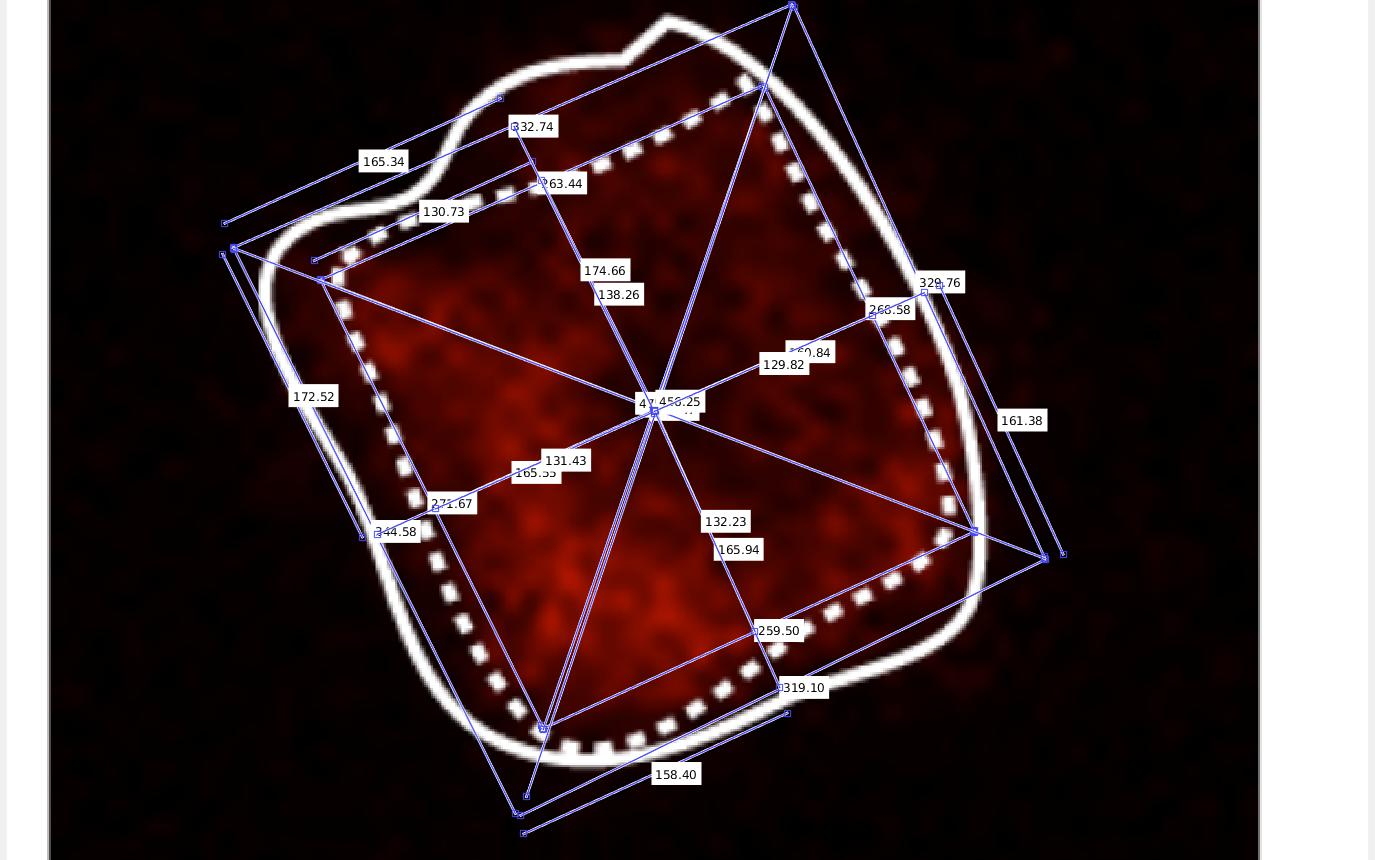
\includegraphics[width=0.5\linewidth,height=0.3\textheight]{../Images/patchExpansion/patchExpansionMeasurement}
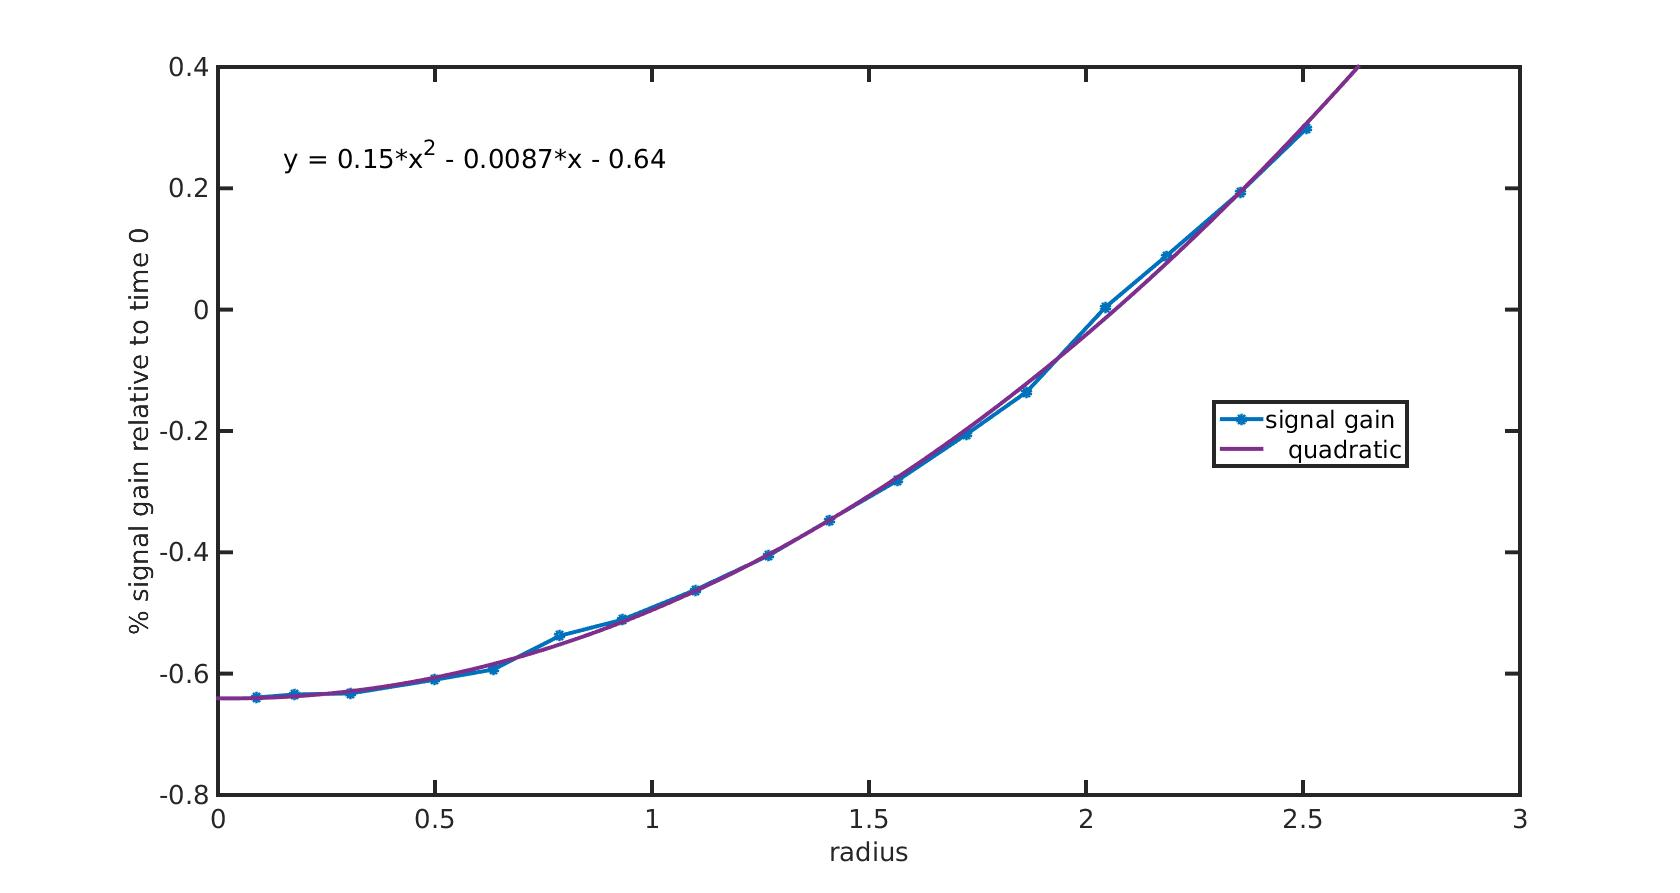
\includegraphics[width=0.5\linewidth, height=0.3\textheight]{../Images/patchExpansion/nucleosomeSignalGainConcentricFit}
\caption{The histone patch (left) at time 0 (dashed line) and 15 minutes post UVC (full line). The relative gain function $y(r)$ and a quadratic fit up to the boundary of the patch at time 0 (right)}
\label{fig:nucleosomeSignalGainConcentricFit}
\end{figure}

The amount of histones between $r$ and $r+dr$ is given by 
\begin{equation*}
F(r) \propto r
\end{equation*}

We define a function $g(r_i)$, which indicates the percentage of signal transfered due to sliding and expansion from concentric ring at $r_i$ to $r_{i+1}$ given the signal received from $r_{i-1}$. In practice, we do not have knowledge of the amount of signal transfered from one ring to the next, but only the resulting signal, 15 minutes post UVC. 

We further assume that the expansion starts from the inner-most ring and spreads outwards. Using the gain function $y(r)$, the amount of signal left in the first ring 15 minutes post UVC is
\begin{equation*}
F(r_1)(1+g(r_1)) = F(r_1)(1+y(r_1)) \Rightarrow g(r_1)=y(r_1)
\end{equation*}
The second ring receives $-g(r_1)F(r_1)$ from the first ring, and gains $g(r_2)$ fraction of the total it has. 
\begin{equation*}
(F(r_2)-g(r_1)F(r_1))(1+g(r_2))= F(r_2)(1+y(r_2))
\end{equation*}
Therefore, 
\begin{equation*}
 g(r_2)=\frac{F(r_1)y(r_1)+F(r_2)y(r_2)}{F(r_2)-y(r_1)F(r_1)}
\end{equation*}

Continuing in this manner, we have for $g(r_k)$
\begin{equation}\label{eq:survivalFunctionDiscrete}
g(r_k) =\frac{\sum_{i=1}^k F(r_i)y(r_i)}{F(r_k)-\sum_{j=1}^{k-1}y(r_j)F(r_j)} 
\end{equation} 

For infinitesimally small $dr$, the sums in equation \ref{eq:survivalFunctionDiscrete}, can be transformed into an integral form, and $r_1,r_2,..,r_N$ to a continues variable in the range $r\in [0, R]$

\begin{equation}\label{eq:survivalFunctionContinuous}
g(r) =\frac{\int_{0}^r F(\phi)y(\phi)d\phi}{F(r)-\int_{0}^{r}y(\phi)F(\phi)d\phi} 
\end{equation}

We note that
\begin{equation*}
1+g(r) =\frac{F(r)}{F(r)-\int_0^r y(\phi)F(\phi)d\phi}
\end{equation*}
is the ratio of particles remaining is ring $r$ to those existing in $r$. We can use this function to calculate the probability that a particle which omit a signal is found at a distance larger than $r$ from its initial position. For this end, we can estimate the survival function 
\begin{equation*}
S(r)=\prod_r (1+g(r)) =\prod_r \frac{F(r)}{F(r)-\int_0^r y(\phi)F(\phi)d\phi}
\end{equation*}


substituting the forms of functions
\begin{equation*}
F(r)=r, \quad y(r) =0.15r^2 -0.0087r-0.64
\end{equation*}
 we get, after performing integration and rearranging
\begin{equation}
S(r) =	\prod_r \frac{1}{1-0.15r^3/4 +0.0087r^2/3 +0.64r/2}
\end{equation}

 
\end{document}